\documentclass[11pt]{article}
\usepackage{graphicx}
\usepackage{float}
\usepackage{amsmath}
\usepackage{amsfonts}
\usepackage[brazilian]{babel}
\usepackage[utf8]{inputenc}
\usepackage[T1]{fontenc}

\begin{document}

\title{Trigonometria}
\author{Erik Perillo}
\date{}
\maketitle

\newpage

\tableofcontents

\newpage

\section{O que é trigonometria?}
\paragraph{}
Trigonometria é a área da matemática que estuda as relações existentes em 
triângulos. Isso se mostrará muito útil em várias áreas da engenharia.
Embora simples, a trigonometria é extremamente poderosa e já possibilitou 
à humanidade, por exemplo, calcular o raio da Terra.

\section{Triângulos}
Os triângulos têm uma propriedade muito interessante:
\textbf{A soma dos ângulos internos de um triângulo é sempre 180 graus}.
Não é possível você fazer um triângulo que não segue essa regra.

\subsection{Tipos de triângulo}
\paragraph{}
Triângulos podem ser classificados de diversas maneiras, mas aqui vamos nos
importar com apenas algumas delas. Vamos olhar os ângulos internos do triângulo
para dar a eles rótulos. Os tipos que consideraremos são:
\begin{itemize}
	\item Triângulo acutângulo: Os ângulos internos são todos \textbf{menores}
		que 90 graus.
	\item Triângulo retângulo: Um dos ângulos tem 90 graus.
	\item Triângulo obtusângulo: Um dos ângulos tem mais de 90 graus.
\end{itemize}

Abaixo temos uma ilustração bonitinha que mostra as diferenças.
\begin{figure}[H]
	\centering
	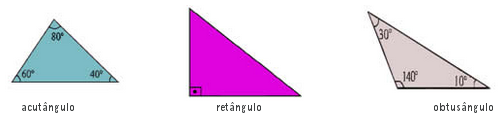
\includegraphics[width=1.0\linewidth]{imgs/tipos_triangulos.png}
\end{figure}

\subsection{Triângulos Retângulos}
\paragraph{}
Dentre os tipos que vimos, o tipo mais importante é o triângulo retângulo. 
Ele tem propriedades muito interessantes que vamos aprender a seguir.
\par
O Triângulo retângulo tem nomes especiais para suas partes:
\begin{itemize}
	\item Catetos: os lados do triângulo que tocam o ângulo reto.
	\item Hipotenusa: o lado do triângulo que \textbf{não} toca o ângulo reto.
\end{itemize}
\begin{figure}[H]
	\centering
	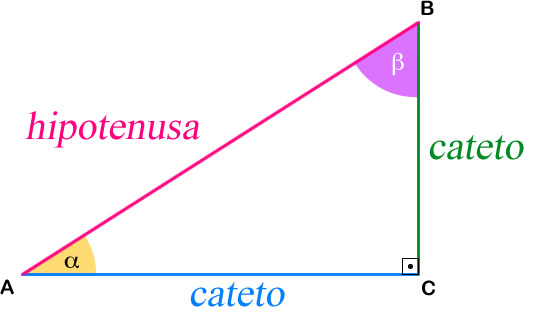
\includegraphics[width=0.5\linewidth]{imgs/lados.jpg}
	\caption{Nomes dos lados do triângulo}
\end{figure}
A partezinha quadrada com um ponto indica que este é um ângulo reto, ou seja,
de 90 graus.

\section{O teorema de Pitágoras}
\paragraph{}
Os ângulos \emph{retângulos} (e apenas esses) têm uma propriedade muito legal:
\textbf{A soma dos quadrados dos catetos é igual ao quadrado da hipotenusa}.
Olhando para a figura a seguir, damos os nomes de a, b, e c para os lados 
do triângulo retângulo:
\begin{figure}[H]
	\centering
	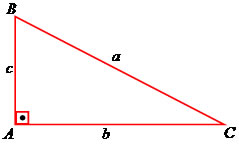
\includegraphics[width=0.5\linewidth]{imgs/trig_ret.jpg}
\end{figure}
Seguindo a regra que acabamos de dar, então, é verdade que:
$$b^2 + c^2 = a^2$$
Vamos fazer um exemplo? Faça no papel, com a ajuda de uma régua, um triângulo 
retângulo de catetos de $3$ e $4$ cm. Segundo o teorema de pitágoras, qual
o tamanho da hipotenusa? Oras, tem que ser:
$$h^2 = 3^2 + 4^2 \implies h^2 = 9 + 16 \implies h^2 = 25 \implies h = 5$$
Desenhe agora a hipotenusa. Pode checar com a régua, deu exatamente $5$cm!

\section{Senos, cossenos e tangentes}
\paragraph{}
Senos e cossenos são muito importantes. Todo seno está associado a um ângulo.
Considere a figura a seguir:
\begin{figure}[H]
	\centering
	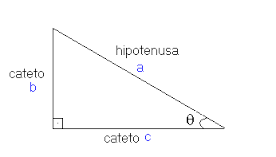
\includegraphics[width=0.5\linewidth]{imgs/seno.png}
\end{figure}
Então temos as seguintes relações:
\begin{itemize}
	\item $sen(\theta)$ (seno de $\theta$) = 
		\textbf{cateto oposto sobre a hipotenusa} = $\frac{b}{a}$
	\item $cos(\theta)$ = 
		\textbf{cateto adjacente sobre a hipotenusa} = $\frac{c}{a}$
	\item $tan(\theta)$ = 
		\textbf{cateto oposto sobre o adjacente} = $\frac{b}{c}$
\end{itemize}

\newpage

\section{Exercícios}
\begin{enumerate}
	\item Determine o valor de x para os triângulos a seguir:
		\begin{enumerate}
			\item --
				\begin{figure}[H]
					\centering
					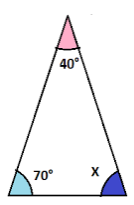
\includegraphics[width=0.3\linewidth]{imgs/ex1.png}
				\end{figure}
			\item --
				\begin{figure}[H]
					\centering
					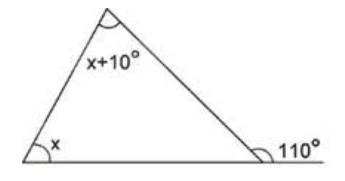
\includegraphics[width=0.5\linewidth]{imgs/ex2.png}
				\end{figure}
			\item --
				\begin{figure}[H]
					\centering
					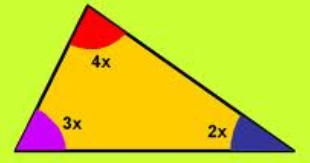
\includegraphics[width=0.5\linewidth]{imgs/ex3.png}
				\end{figure}
		\end{enumerate}

	\item O senhor Parker precisa fazer uma teia até a ponta de seu prédio
		Favorito, como ilustrado abaixo.
		\begin{figure}[H]
			\centering
			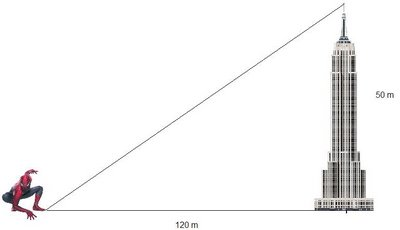
\includegraphics[width=0.8\linewidth]{imgs/spid.jpg}
		\end{figure}
		Supondo que o prédio tem 50 metros de altura e a distância
		do Parker até o prédio é de 120 metros, quantos metros tem que ter a 
		sua teia?

	\item Considere a imagem a seguir:
		\begin{figure}[H]
			\centering
			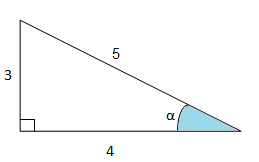
\includegraphics[width=0.5\linewidth]{imgs/boa.png}
		\end{figure}
		Qual é o valor de:
		\begin{itemize}
			\item Seno de $\alpha$?
			\item Cosseno de $\alpha$?
			\item Tangente de $\alpha$?
		\end{itemize}
\end{enumerate}

\newpage

\section{Respostas aos Exercícios}
\begin{enumerate}
	\item 
		\begin{enumerate}
			\item A soma dos ângulos dos triângulos é sempre 180 graus.
				$$40 + 70 + x = 180 \implies x = 180 - 40 - 70 = 70$$
			\item $$(x + 10) + x + (180 - 110) = 180$$
				$$2x + 80 = 180 \implies 2x = 100 \implies x = 50$$
			\item $$4x + 3x + 2x = 180 \implies x*(4 + 3 + 2) = 180$$
				$$9x = 180 \implies x = 180/9 = 20$$
		\end{enumerate}

	\item Notando que a algura do prédio é um cateto (vamos chamar de b) 
		e a distância do homem aranha até o prédio é um cateto também
		(vamos chamar de c), então temos que a hipotenusa (chamando de h) é:
		$$h^2 = b^2 + c^2$$
		$$h^2 = {(50)}^2 + {(120)}^2 = 16900$$
		$$h = \sqrt{16900} = 130$$

	\item
		\item $sen(\alpha) = \frac{3}{5}$
		\item $cos(\alpha) = \frac{4}{5}$
		\item $tan(\alpha) = \frac{3}{4}$
\end{enumerate}

\end{document}
